OpenQuake allows the time period for which the loss exceedance probabilities are calculated to be different from the time period associated with the hazard curve calculation. The hazard curve is calculated for a time period of 50 years, and the loss curve is calculated for a time period of 75 years.

Table~\ref{tab:vf-ln-tax1-nzcov} shows the mean loss ratios and corresponding coefficients of variation for the vulnerability function used in this test case.

\begin{table}[htbp]

\centering
\tabcolsep=0.11cm
\scalebox{0.6}{

\begin{tabular}{ l c c c c c c c c c c c }

\hline
\rowcolor{anti-flashwhite}
\bf{PGA} & \bf{0.05g} & \bf{0.20g} & \bf{0.40g} & \bf{0.60g} & \bf{0.80g} & \bf{1.00g} & \bf{1.20g} & \bf{1.40g} & \bf{1.60g} & \bf{1.80g} & \bf{2.00g} \\
\hline
\bf{P.O.E.} & 8.643\times10^{-1} & 7.171\times10^{-1} & 4.371\times10^{-1} & 2.364\times10^{-1} & 1.234\times10^{-1} & 6.427\times10^{-2} & 3.382\times10^{-2} & 1.802\times10^{-2} & 9.676\times10^{-3} & 5.192\times10^{-3} & 2.748\times10^{-3}\\
\hline
\end{tabular}

}

\caption{50-year hazard curve for PGA at a single site}
\label{tab:hc-l1-50}
\end{table}

The intensity levels for the hazard curve are extracted from the vulnerability function: $[0.05, 0.20, 0.40, 0.60, 0.80, 1.00, 1.20, 1.40, 1.60, 1.80, 2.00]$. The hazard curve gives the probabilities of exceedance for a set of intensity levels within a specified time period. The time period in this case, $t_H$, is fifty years. The hazard curve at the location of the single asset used in this test case is shown in Table~\ref{tab:hc-l1-50}.

The probabilities of exceedance are: $[8.643\times10^{-1}, 7.171\times10^{-1}, 4.371\times10^{-1}, 2.364\times10^{-1}, 1.234\times10^{-1}, 6.427\times10^{-2}, 3.382\times10^{-2}, 1.802\times10^{-2}, 9.676\times10^{-3}, 5.192\times10^{-3}, 2.748\times10^{-3}]$. The probabilities of exceedance are first converted to annual rates (or frequencies) of exceedance by employing the Poissonion conversion:

\begin{equation}
	\lambda(iml) = \frac{-\ln [1 - prob(IML > iml, t_H)]}{t_H}
\end{equation}

The annual frequencies of exceedance are: $[3.994\times10^{-2}, 2.525\times10^{-2}, 1.149\times10^{-2}, 5.394\times10^{-3}, 2.633\times10^{-3}, 1.329\times10^{-3}, 6.881\times10^{-4}, 3.636\times10^{-4}, 1.945\times10^{-4}, 1.041\times10^{-4}, 5.504\times10^{-5}]$.

The annual frequencies of occurrence are estimated by the differentiation of the annual frequencies of exceedance: $[1.469\times10^{-2}, 1.376\times10^{-2}, 6.101\times10^{-3}, 2.760\times10^{-3}, 1.305\times10^{-3}, 6.404\times10^{-4}, 3.245\times10^{-4}, 1.692\times10^{-4}, 9.035\times10^{-5}, 4.907\times10^{-5}]$.

The loss ratios at which the loss curve exceedance probabilities are calculated are obtained from the vulnerability function and the parameter `steps\_per\_interval'. The default value of `steps\_per\_interval' is one, which is the value used in this case. The loss ratios in the vulnerability function are $[0.01, 0.04, 0.10, 0.20, 0.33, 0.50, 0.67, 0.80, 0.90, 0.96, 0.99]$.

The vulnerability model is then transformed into a matrix describing probabilities of exceedance for the selected set of loss ratios conditional on the set of ground motion intensity levels. Since there is no variability in the loss ratio, calculation of the loss curves is straightforward in this case. Since the coefficients of variation in the vulnerability function are all zero, the lognormal distribution devolves into the degenerate distribution. The loss ratio exceedance matrix in this case is shown in Table~\ref{tab:lrem-ln-tax1-nzcov-75}.

\begin{table}[htbp]

\centering
\begin{tabular}{ l c c c c c c c c c }

\hline
\rowcolor{anti-flashwhite}
\bf{LR | PGA} & \bf{0.05g} & \bf{0.20g} & \bf{0.40g} & \bf{0.60g} & \bf{0.80g} & \bf{1.00g} & \bf{1.20g} & \bf{\dots} & \bf{2.00g} \\
\hline
\bf{0.01} & 0.494 & 1.000 & 1.000 & 1.000 & 1.000 & 1.000 & 1.000 & \dots & 1.000 \\
\bf{0.04} & 0.000 & 0.476 & 1.000 & 1.000 & 1.000 & 1.000 & 1.000 & \dots & 1.000 \\
\bf{0.10} & 0.000 & 0.000 & 0.453 & 0.980 & 0.999 & 1.000 & 1.000 & \dots & 1.000 \\
\bf{0.20} & 0.000 & 0.000 & 0.001 & 0.438 & 0.881 & 0.986 & 0.999 & \dots & 1.000 \\
\bf{0.33} & 0.000 & 0.000 & 0.000 & 0.039 & 0.427 & 0.812 & 0.959 & \dots & 1.000 \\
\bf{0.50} & 0.000 & 0.000 & 0.000 & 0.001 & 0.094 & 0.424 & 0.730 & \dots & 1.000 \\
\bf{0.67} & 0.000 & 0.000 & 0.000 & 0.000 & 0.017 & 0.170 & 0.427 & \dots & 1.000 \\
\bf{0.80} & 0.000 & 0.000 & 0.000 & 0.000 & 0.005 & 0.079 & 0.253 & \dots & 1.000 \\
\bf{0.90} & 0.000 & 0.000 & 0.000 & 0.000 & 0.002 & 0.043 & 0.162 & \dots & 0.999 \\
\bf{0.96} & 0.000 & 0.000 & 0.000 & 0.000 & 0.001 & 0.030 & 0.122 & \dots & 0.844 \\
\bf{0.99} & 0.000 & 0.000 & 0.000 & 0.000 & 0.001 & 0.025 & 0.106 & \dots & 0.494 \\
\bf{1.00} & 0.000 & 0.000 & 0.000 & 0.000 & 0.001 & 0.023 & 0.101 & \dots & 0.363 \\
\hline
\end{tabular}

\caption{Conditional loss ratio exceedance matrix for classical risk test case 3a}
\label{tab:lrem-ln-tax1-nzcov-75}
\end{table}

Now, the sum product of each row of the conditional loss ratio exceedance matrix with the annual frequencies of occurrence of the respective intensity levels gives the annual frequency of exceedance for the respective loss ratios. The loss ratio annual frequencies of exceedance thus calculated are: $[3.988\times10^{-2}, 3.617\times10^{-2}, 2.509\times10^{-2}, 1.280\times10^{-2}, 5.654\times10^{-3}, 2.765\times10^{-3}, 1.408\times10^{-3}, 7.772\times10^{-4}, 4.896\times10^{-4}, 3.276\times10^{-4}, 2.457\times10^{-4}, 2.037\times10^{-4}, 1.903\times10^{-4}]$.

The probabilities of exceedance of the set of loss ratios are obtained by converting the annual frequencies of exceedance back into probabilities of exceedance over 75 years by using the Poissonion equation. The loss curve probabilities of exceedance for a time period of 75 years are: $[9.498\times10^{-1}, 9.336\times10^{-1}, 8.477\times10^{-1}, 6.170\times10^{-1}, 3.456\times10^{-1}, 1.873\times10^{-1}, 1.002\times10^{-1}, 5.663\times10^{-2}, 3.606\times10^{-2}, 2.427\times10^{-2}, 1.826\times10^{-2}, 1.516\times10^{-2}, 1.417\times10^{-2}]$.

The loss curve thus calculated above is compared with the loss curve obtained using the OpenQuake classical PSHA based risk calculator in Figure~\ref{fig:lc-cr-3a}.

\begin{figure}[htbp]
\centering
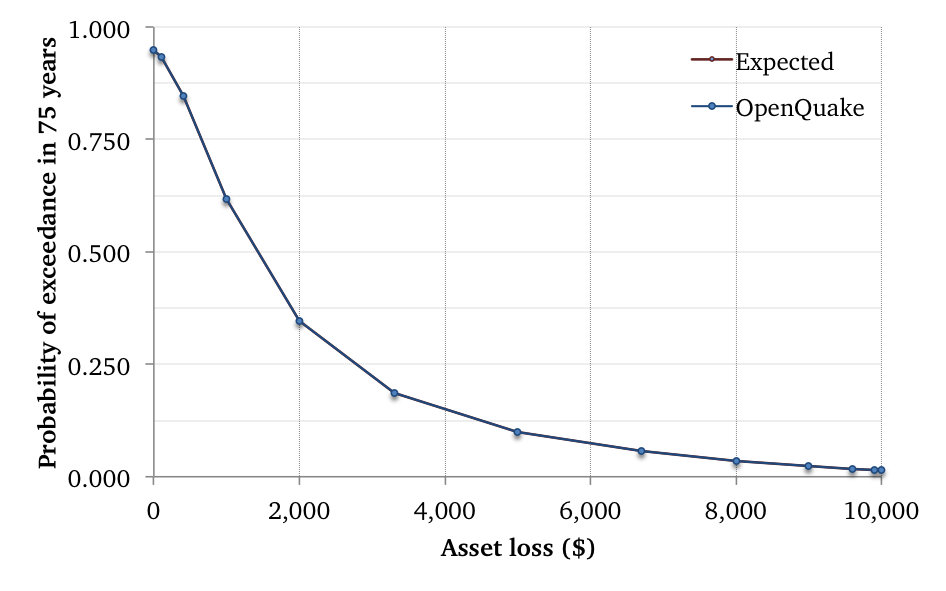
\includegraphics[width=12cm]{qareport/figures/fig-lc-cr-3a}
\caption{Loss curve comparison for classical risk test case 3a}
\label{fig:lc-cr-3a}
\end{figure}

The area under the loss exceedance curve gives the expected loss over 75 years.
